\chapter{High(er) performance Python}
\label{chapter:performance}
\begin{center}
  {\Large\textit{\\ \vspace{0.1in} - }}
\end{center}
\vspace{0.2in}

To many people, high performance scientific code \emph{must} be written in a language such as C/C++ or Fortran (or even a GPU language).  It is true that these languages will continue to support applications where the highest possible performance is absolutely essential.  For example, some climate simulations can take months of time on a supercomputer, and therefore even a modest 2x speedup of code can make a huge difference.  However, this is not always the case.  In the authors' experience, the time spent writing code (a.k.a. \emph{developer time}) usually far exceeds the time spent waiting for a computer to crunch numbers (a.k.a. \emph{CPU time}).   Since python code is generally easier to write and maintain than e.g. C++, the project goal (e.g. predicting an outcome) can be achieved far quicker and cheaper using Python.  Moreover, Python does not require a developer to mange low-level tasks such as memory allocation, so a non-expert programmer (e.g. a person with a PhD in statistics) can often be used.

The fact that python does not require a programmer to manage memory allocation does not mean that a fundamental understanding of computer engineering will not help.  Used carelessly and without attention to computational limitations, Python can be a very very slow language.

In this chapter we present some basic computer engineering concepts and show how the relate to Python performance.  We also present a number of practical examples of what can be done to increase performance of your code.

\section{Memory hierarchy}
One can think of a computer as a machine that takes data from disk and transfers it to a CPU.  The CPU, which is composed of a control unit, arithmetic logic unit, and more, transforms this data, which is then written back to disk or displayed to the user.  The term \emph{memory hierarchy} refers to the hierarchical storage scheme for data.  See figure \ref{performance:fig:heirarchy1} for a simplified version that shows memory getting smaller and faster (in terms of the time needed to access it) as you get closer to the CPU core.  In figure \ref{performance:fig:heirarchy1} we measure time in CPU clock cycles.  The CPU clock is a source of electrical pulses that synchronize CPU operations.  As of 2013, typical laptop CPU clocks operate at 2-3 billion cycles per second (GHz). The reasons why the larger memory is slower has to do with a combination of economics and physics and is beyond the scope of this text.  Note that the actual memory hierarchy is more complicated with multiple levels of cache and registers (figures \ref{performance:fig:pyramid}, \ref{performance:fig:heirarchy3}).).

\begin{figure}
  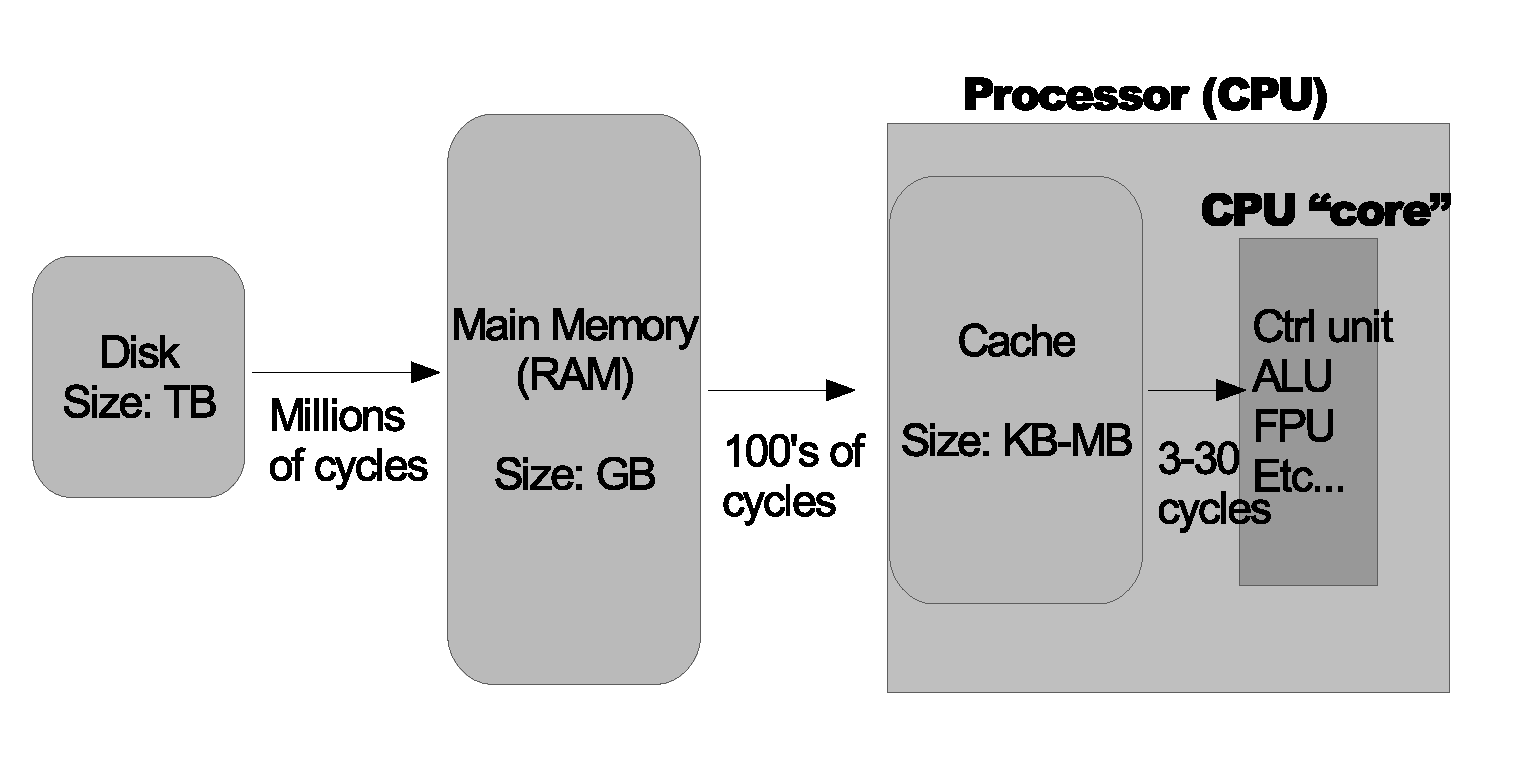
\includegraphics[width=0.9\textwidth]{../images/memory_heirarchy}
  \caption{Simplified memory hierarchy showing disk, main memory (RAM), cache, the computer components they are situated in, and the time (in clock cycles) needed to move data between them.}
  \label{performance:fig:heirarchy1}
\end{figure}
\begin{figure}
  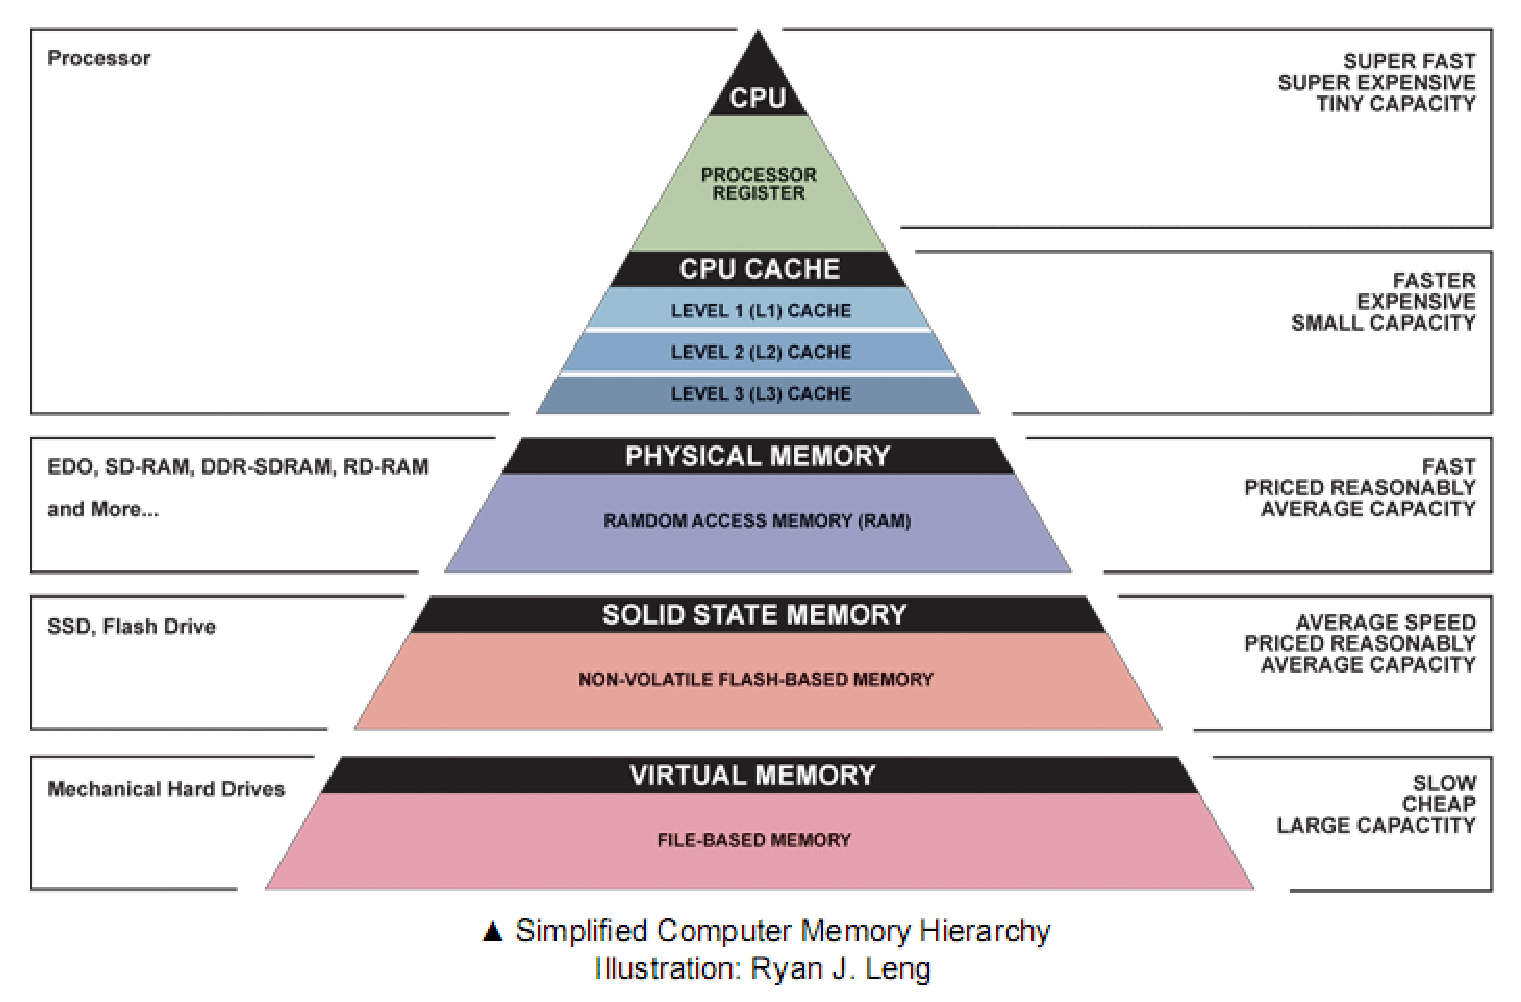
\includegraphics[width=0.85\textwidth]{../images/hei}
  \caption{Memory hierarchy with more detail.}
  \label{performance:fig:pyramid}
\end{figure}
\begin{figure}
  
\includegraphics[width=0.85\textwidth]{../images/haswelldiemap_550}
  \caption{Picture of an Intel core i7 chip showing shared L3 cache.  L1 and L2 cache as well as registers are located on the CPU core.}
  \label{performance:fig:heirarchy3}
\end{figure}
What you need to keep in mind is that if the slower component cannot supply the faster upstream component with data, then we have a bottleneck.  This \emph{memory wall} can only be avoided with one of two means.  First, the faster upstream component can make repeated use of its data.  For example, you can load a training data set from disk into memory and use it to train a logistic regression.  The loading of the data is slow because of the disk access.  However, this happens only once, and then (for at least a few minutes) the data is repeatedly used in an optimization procedure.  The access time difference between main memory and cache can be mitigated in a similar manner.  
% TODO Put in a gemm example
Take for example the \emph{axpy} operation $z = ax + y$ where $x$ and $y$ are vectors and $a$ is a scalar.  It often happens that $x$ and $y$ are too large to fit in cache.  One wrong way to deal perform the axpy would be to first load as much of $x$ as possible into cache, multiply it by $a$, then send that result back to memory and load the next bit of $x$ in.  After we had multiplied $ax$, we could start loading both $ax$ and $y$ into cache and add them.  A smarter implementation loads smaller chunks of $x$ and $y$ so that they fit into cache.  We then multiply the chunk of $x$ by $a$ and then add it to that chunk of $y$.  This ``double usage'' of $x$ avoids one cache-memory load and speeds code up the axpy operation significantly.

%A similar phenomenon happens with main memory and cache.  Take for example computing the dot product between two vectors $x\cdot y = \sum_ix_iy_i$.  If the vectors both fit into cache, then we can load both into cache, multiply them together, then add the result.  If however they do not fit, it makes sense to divide $x$ and $y$ into $n$ length $m$ chunks such that each chunk of $x$ and $y$ fit into memory together.  We can then do the dot product on every chunk independently and then add the result.  For example, writing the first $x$ chunk as $(x_{11},\cdots,x_{1m})$, and the $n^{th}$ we $(x_{n1},\cdots,x_{nm})$, we then decompose the dot product as:
%\begin{align}
%  x\cdot y &= \left( x_{11}y_{11} + \cdots x_{1m}y_{1m} \right) + \cdots + (x_{n1}y_{n1} + \cdots x_{nm}y_{nm}).
%  \label{performance:align:dotprod}
%\end{align}
The second means to avoid a memory wall is to slow down the CPU clock.  Since the clock runs slower, the slower components take less CPU cycles to do their work, and thus less cycles are wasted.  This by itself does not help performance.  However, the slower clock speeds consume far less power, and allow more cores (each with their own cache) to be placed on chip.  The overall performance increases, but comes at the cost of added complexity (programmers need to design parallel algorithms).  This sort of clock-slowing became more-or-less inevitable when (for years) CPU clock speeds increased at a much higher rate than memory bus speeds.

One final note on memory.  While the casual programmer generally thinks very little about main memory vs. cache vs. registers, he or she absolutely needs to be aware of disk versus main memory.  If your computer cannot fit all data in main memory, it will use a portion of the disk, called \emph{swap space} as a kind of pseudo memory.  Since reading/writing to and from disk is exceptionally slow, this practice of \emph{swapping} can significantly slow down all operations on your computer.  This can crash servers.  For this reason, it is your responsibility to keep track of memory usage.  While all machines have built in utilities that do this, the ``best'' one is \T{htop}\footnote{\T{htop} does not work on all versions of mac.  There are \T{htop} installers, but sometimes the memory usage just doesn't make sense.}  In Ubuntu you can install with \T{sudo apt-get install htop}.  You can start the utility by typing \T{htop} in the command prompt.  In addition to monitoring memory usage, \T{htop} allows you to see CPU usage, kill processes, and search for processes.

\begin{figure}
  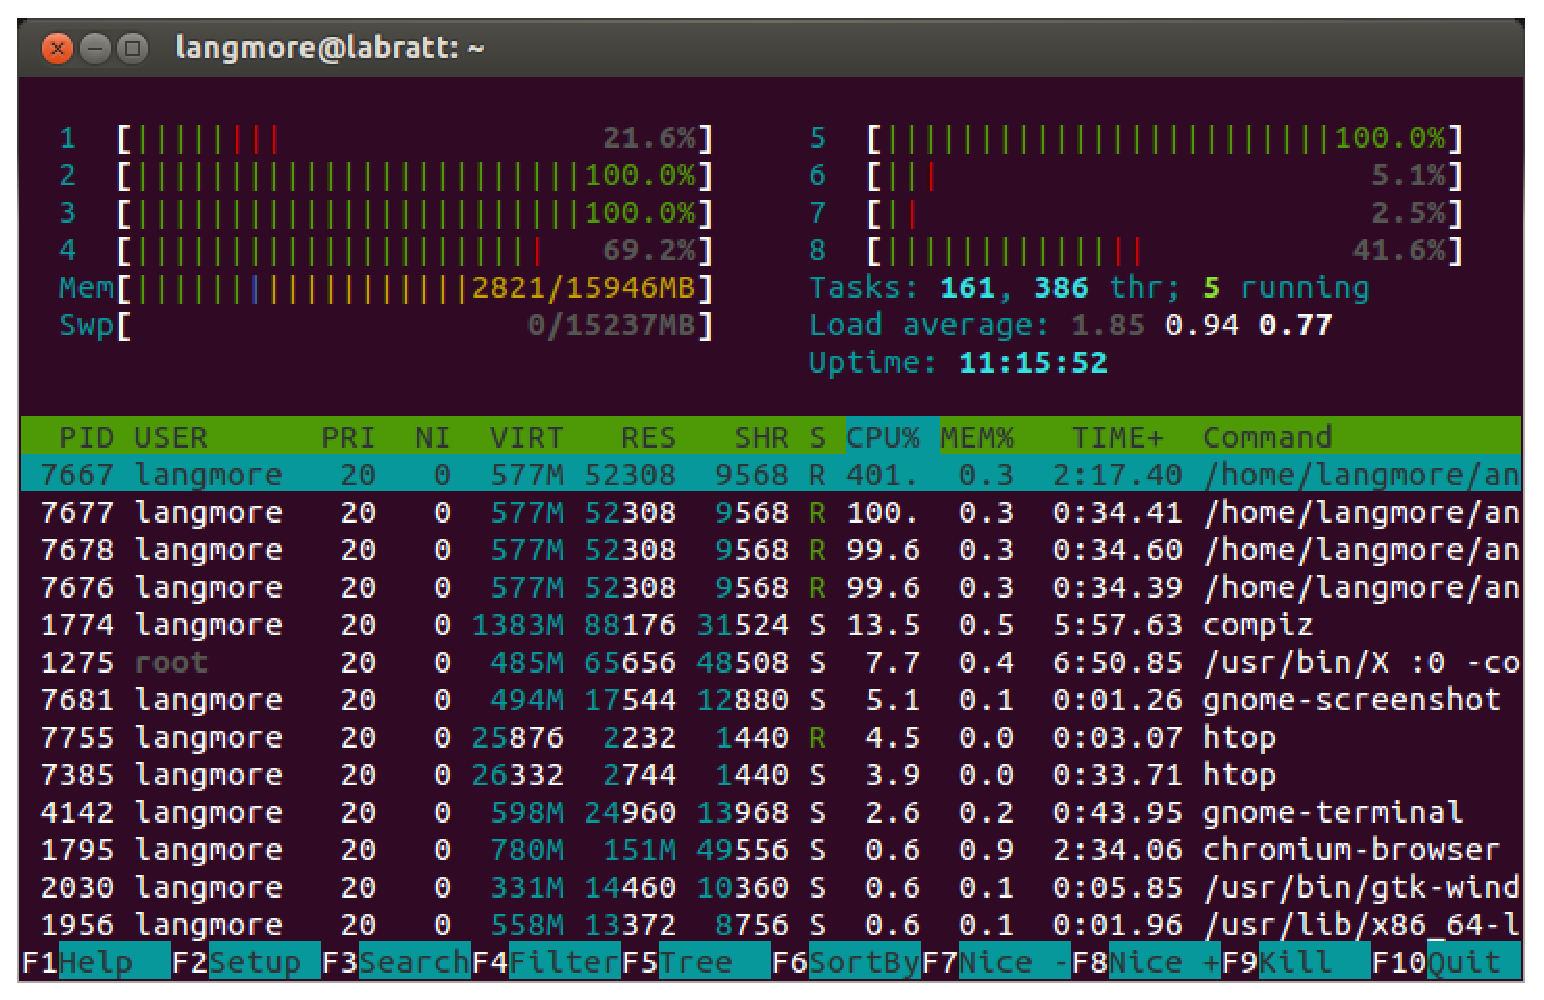
\includegraphics[width=\textwidth, clip=True, trim=0 100 0 0]{../images/htop}
  \caption{Screenshot of \T{htop} invoked on a laptop with 4 cores and 4 virtual cores (so it appears as 8 cores to the OS).  Notice that multiple cores are in use due to a multi-threaded numpy matrix multiply.  You can also see that 2821 MB of memory is currently in use.  The green memory and CPU usage is ``normal usage'', and red indicates ``kernel usage'', in other words, the OS kernel is invoking this.  The most common example of a red CPU line is due to a disk read/write.}
  \label{performance:fig:htop}
\end{figure}

A useful number to keep in mind when calculating memory usage is to realize that double precision numbers (the default for Python if your system is 64 bit) take up 64 bits, which is 8 bytes.  So an array of numbers that has length 1 million is 8 million bytes, or, 8 MB.

\section{Parallelism}

Since, as we saw above, performance gains will not come through increasing the clock speed in the serial pathway of figure \ref{performance:fig:heirarchy1}, it is now coming through parallelism.  Suppose you have a processor with 4 cores and wish to perform the axpy operation $z = ax + y$.  A starting point could be to divide the memory address range of $x$ and $y$ into four chunks, and send each chunk to a different core.  Each core performs an axpy on each chunk, and then writes the result to the appropriate space in memory (so that the end result is a contiguous array $z$).  If each chunk fits perfectly into each core's cache, and our memory controller can handle these four operations efficiently, then we should see a four-times speedup!  This sort of operation is known as \emph{embarrassingly parallel} because it did not involve communication between the separate cores.

As another example of an embarrassingly parallel algorithm, consider the random forest.  In this case we have $n$ independent trees, each being fit independently (see figure \ref{performance:fig:RF}).
\begin{figure}
  \includegraphics[width=\textwidth]{../images/RF}
  \caption{Random forest is an embarrassingly parallel algorithm.}
  \label{performance:fig:RF}
\end{figure}

As an example of an algorithm that is not embarrassingly parallel, consider solving the system $Ax = b$.  As mentioned in \ref{linear:subsection:numerical}, for medium to large systems this is usually done with algorithms that repeatedly multiply $A$ by different vectors $v$, and then add this result to another vector $w$.  Suppose our machine has two cores.  Then each multiplication can be decomposed as:
\begin{align}
  \label{performance:align:matvec}
  \left( 
  \begin{matrix}
    A_{11} & A_{12}\\
    A_{21} & A_{22}
  \end{matrix}
  \right)
  \left( 
  \begin{matrix}
    v_1\\
    v_2
  \end{matrix}
  \right)
  =
  \left( 
  \begin{matrix}
    A_{11}v_1 + A_{12}v_2 \\
    A_{21}v_1 + A_{22}v_2
  \end{matrix}
  \right)
\end{align}
The first core can handle $A_{11}v_1 + A_{12}v_2$ and thus assemble the top rows of $Av$.  The other core can handle the bottom rows.  However, each result must be sent to the location where the corresponding chunk of $w$ is being kept so that we may compute $Av + w$.  This process repeats many times, and during each repetition, the result must be shared between cores.  This \emph{communication} incurs some overhead, both in terms of programming time and cpu cycles.

More important (at least to our intended audience) than communication overhead is the increase in complexity that comes with parallelizing a program.  Because of this, and the fact that some algorithms cannot be parallelized, large portions of your code will likely remain serial (= not parallel).  If 50\% of your code is serial, then even if you have 1000 cores you can only achieve 50\% speed-up.  This fact is generalized in \emph{Amdahl's law} (see figure \ref{performance:fig:amdahl}).
\begin{figure}
  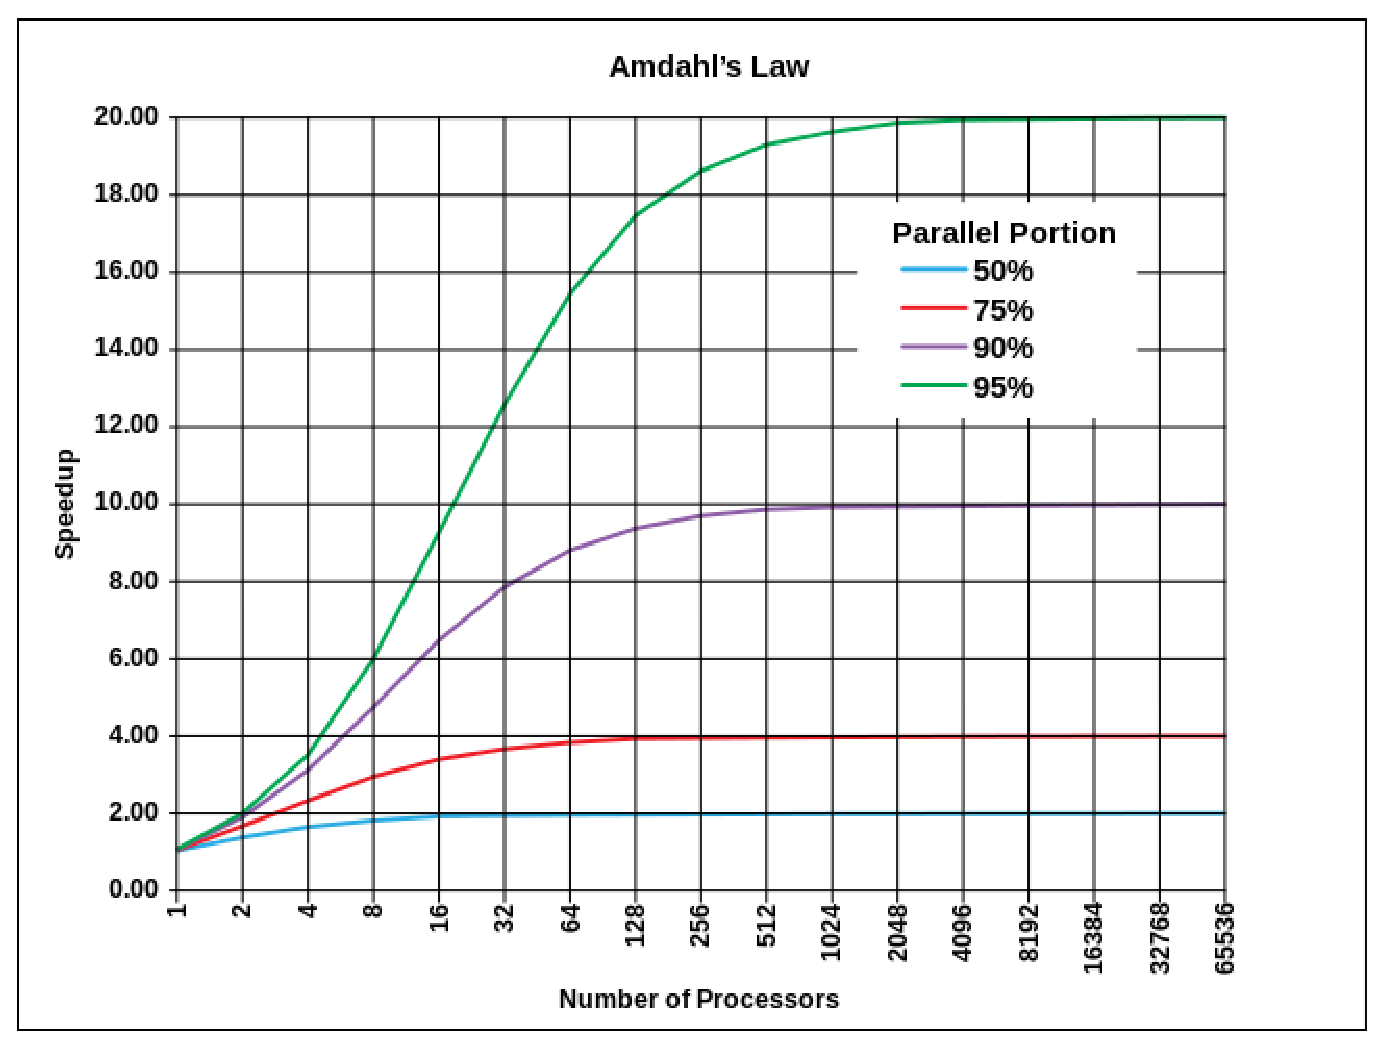
\includegraphics[width=0.5\textwidth]{../images/AmdahlsLaw}
  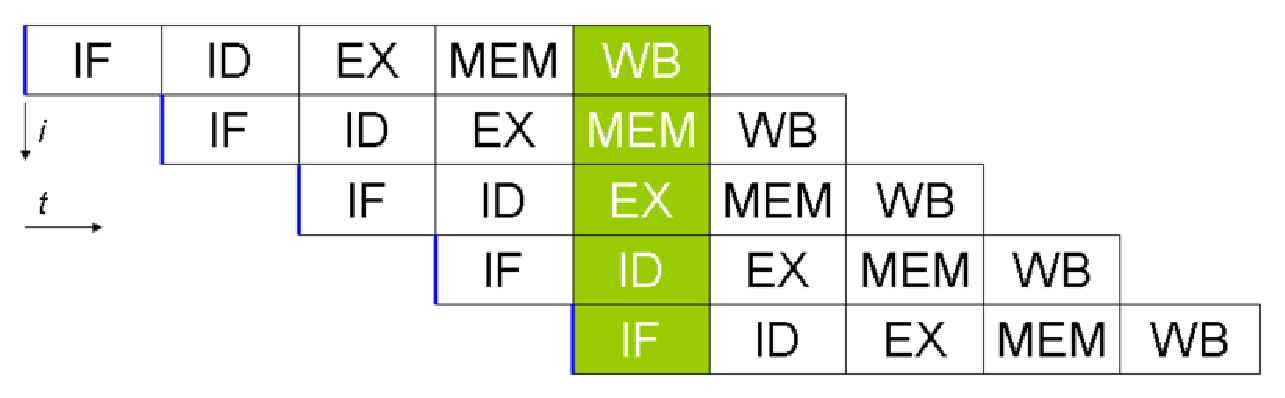
\includegraphics[width=0.5\textwidth]{../images/800px-Fivestagespipeline}
  \label{performance:fig:amdahl}
  \caption{Left:  Amdahl's law states that the fraction of code that is serial places limits on the speedup that parallelization can achieve.  Right: A canonical five-stage pipeline in a RISC machine (IF = Instruction Fetch, ID = Instruction Decode, EX = Execute, MEM = Memory access, WB = Register write back)--cut-and-paste from Wikipedia.}
\end{figure}

It is important to realize that these parallel tasks can be performed by both \emph{processes} and \emph{threads}.  A process is a new ``program'' that is started.  When you start the Firefox web browser, you are starting a new process.  That process has access to its own space in memory.  Python provides support for starting processes through the \emph{subprocess} and \emph{multiprocessing} modules (more on that later).  Since these processes have their own memory space, any data used by them must be copied into that space.  So, for example, if separate processes handled each of the two blocks in \eqref{performance:align:matvec}, then each process would need a \emph{copy} of the data needed to perform that multiplication.  For example, one process would need a copy of $A_{11}$, $A_{12}$, and $v$, and the other process would need a copy of $A_{21}$, $A_{22}$, and $v$.  This can result in unfortunate increase in total memory used.  There are multiple ways to copy data between processes.  In Python, the preferred method is to \emph{serialize} it with the \emph{cPickle} module (turn it into a byte stream) and send using stdin and stdout.  In contrast, multiple \emph{threads} can share a memory space.  This saves memory and eliminates communication overhead.  Threads however are more restricted in what they can do.  For example, if you have two threads running in a Python program, then only one is able to execute code at a time!  This is due to the Global Interpreter Lock (GIL).  This means that multi-threading in Python is very low performance.  

A common library for multi-threading is the Open-MP library.  Due to the GIL, multi-threading directly in Python is not usually done, but libraries such as numpy execute C/Fortran code \emph{outside} of Python and thus avoid the GIL.  In this way, numpy is able to perform parallel programming such as matrix-vector multiplications through multi-threading (thus avoiding the overhead of spawning new processes).  The most popular and versatile multiprocessing library is the Message Passing Interface (MPI).  This library provides a number of ways to start new, and communicate between, processes.  It also provides a number of so-called \emph{reduction} operations whereby data stored on multiple processes is ``reduced'' to one single number.  For example, if each process holds a segment of an array, a possible reduction would involve computing the sum of all the numbers in the array.  The processes each can sum their respective sub-arrays, and then send their result to the master processes, which adds all the sub-sums.  Although MPI is in wide use, it does not provide ways to restart failed tasks.  When you have less than say 100 computers, this is not a big deal.  When however you are Google and regularly perform jobs using thousands of machines, this is important.  For that reason, the \emph{MapReduce} paradigm was developed.  MapReduce allows \emph{mapping} of tasks to individual processes (located on different machines).  It then provides support for different types of reduction as well as restarting of failed tasks.  Hadoop is an open source implementation of MapReduce.  Despite the popularity of Hadoop/MapReduce, it is important to realize that this is a highly restrictive method of parallel computing with a huge overhead required to spawn new processes.

\section{Practical performance in Python}

In this section we introduce you to a few common means to increase the performance of your Python programs.

\subsection{Profiling}

Python code is meant to be easy to understand and maintain.  It is generally \emph{not} good practice to optimize (for performance) everything since this often results in less straightforward code.  To quote Donald Knuth, ``We should forget about small efficiencies, say about 97\% of the time: premature optimization is the root of all evil.''  When you do optimize, the proper first step is to \emph{profile} first.  Profiling is the practice of examining the time taken by different sections of code.  This helps you find the bottlenecks.  You then optimize these bottlenecks.

The easiest way to profile a script is with the unix \T{time} utility.
\begin{minted}{bash}
\$ time python myscript.py

real	0m24.332s
user	0m47.268s
sys	0m0.792s
\end{minted}
The \T{real} line is the total \emph{wall time} of the process invoked directly by the script.  This is the time you would measure if you brought out a stopwatch and timed until the process was finished.  The \T{user} number is the total user CPU time.  In the above case, the script launched a master process, which in turn started two slaves (three processes total).  The master was idle for most of the time, and the slaves worked most of the time.  Therefore, the \T{user} time was about twice the \T{real} time.  The \T{sys} line is the time spent in system calls, such as I/O.

IPython provides a very nice interface to the \emph{timeit} module, which we explain with figure \ref{performance:fig:timeit_1}. In IPython, the timeit module runs the code following the command \T{timeit} (or sometimes, \T{\%timeit} is necessary) a number of times until it has a good estimate of the time needed for it to run.  
\begin{figure}
  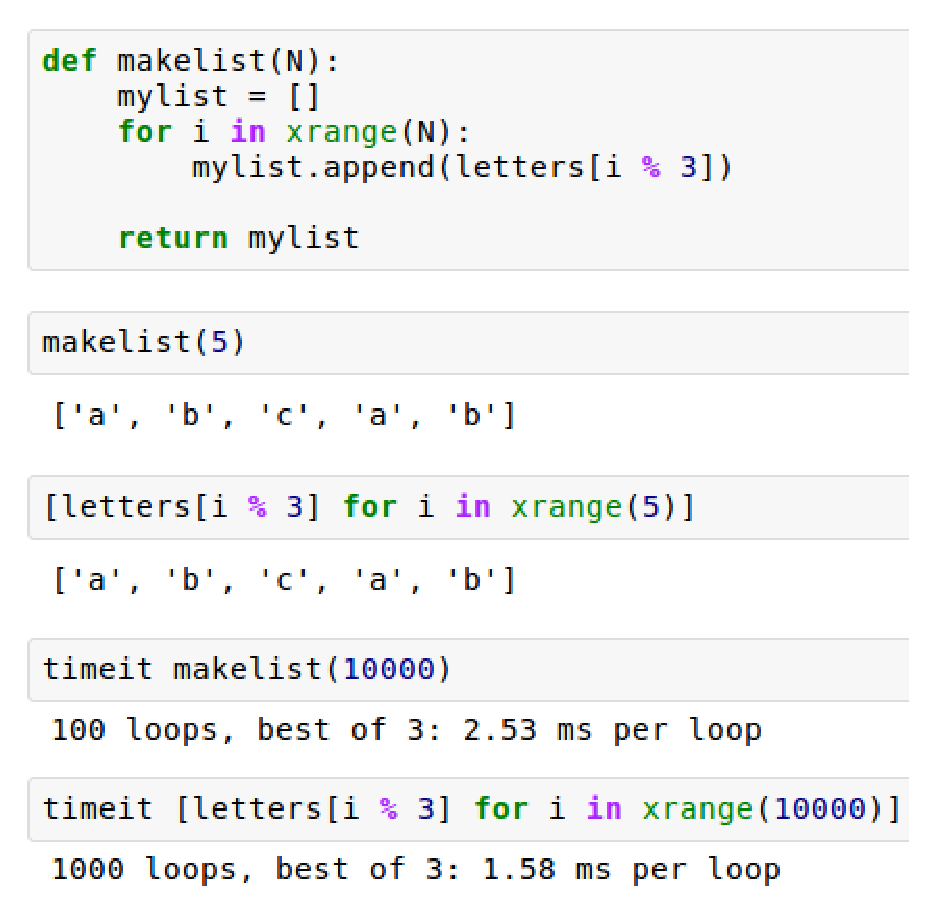
\includegraphics[width=0.7\textwidth]{../images/timeit_1}
  \caption{Figure illustrating use of the timeit module.}
  \label{performance:fig:timeit_1}
\end{figure}
Figure \ref{performance:fig:timeit_1} shows that creating a simple list with 10,000 elements takes about 50\% longer in a for loop than with a list comprehension.  See section \ref{performance:subsection:rulesofthumb} for an explanation of this difference.  Note that \T{timeit} can also be run with the options \T{-n} and \T{-r} which determine the number of iterations used to determine the time the function call takes.

While \T{timeit} can be used to test small snippets of code, it is not the best tool to test larger functions.  The \T{line\_profiler} is the authors' preferred method.  It provides a readout of time spent in each line of a function.  The \T{line\_profiler} can be installed with \T{\$ pip install line\_profiler}.  The easiest way to use the \T{line\_profiler} is to follow these steps (see also listing \ref{performance:listing:lineprofiler}):
\begin{enumerate}
  \item Wrap your code in a function, and then put an \T{@profile} decorator at the top of the function.
  \item Run this function with some command line argument.  This is usually done by writing a script that calls the function (either a unit test, or some script you are using to help run your code).  This script can even be the same module as the function, where you have written ``run capabilities'' into a \T{if \_\_name\_\_ == '\_\_main\_\_':} clause.  
  \item Supposing the script is called \T{myscript.py}, call the script with the command line argument:  \T{kernprof.py -l myscript.py}.  The \T{-l} argument invokes line-by-line profiling\ldots and you will get funny errors if you don't use \T{-l}.
  \item View the results with \T{python -m line\_profiler myscript.py.lprof}.  This prints the results to stdout, so it is often useful to pipe them to \T{less}.
\end{enumerate}
\begin{listing}
  \begin{minted}{python}
import numpy as np

def pythondot(list1, list2):
    dotsum = 0
    for i in xrange(len(list1)):
        dotsum += list1[i] * list2[i]
    
    return dotsum

def numpydot(arr1, arr2):
    return arr1.dot(arr2)

@profile
def testfuns(arrsize, numiter):
    mylist = [1] * arrsize
    myarray = np.ones(arrsize)

    for i in xrange(numiter):
        temp = pythondot(mylist, mylist)
        temp = numpydot(myarray, myarray)

if __name__ == '__main__':
    testfuns(1000, 10) 
  \end{minted}
  \caption{Profiling various dot products with the \T{line\_profiler} module (see also figure \ref{performance:fig:lineprofiler}).}
  \label{performance:listing:lineprofiler}
\end{listing}
\begin{figure}
  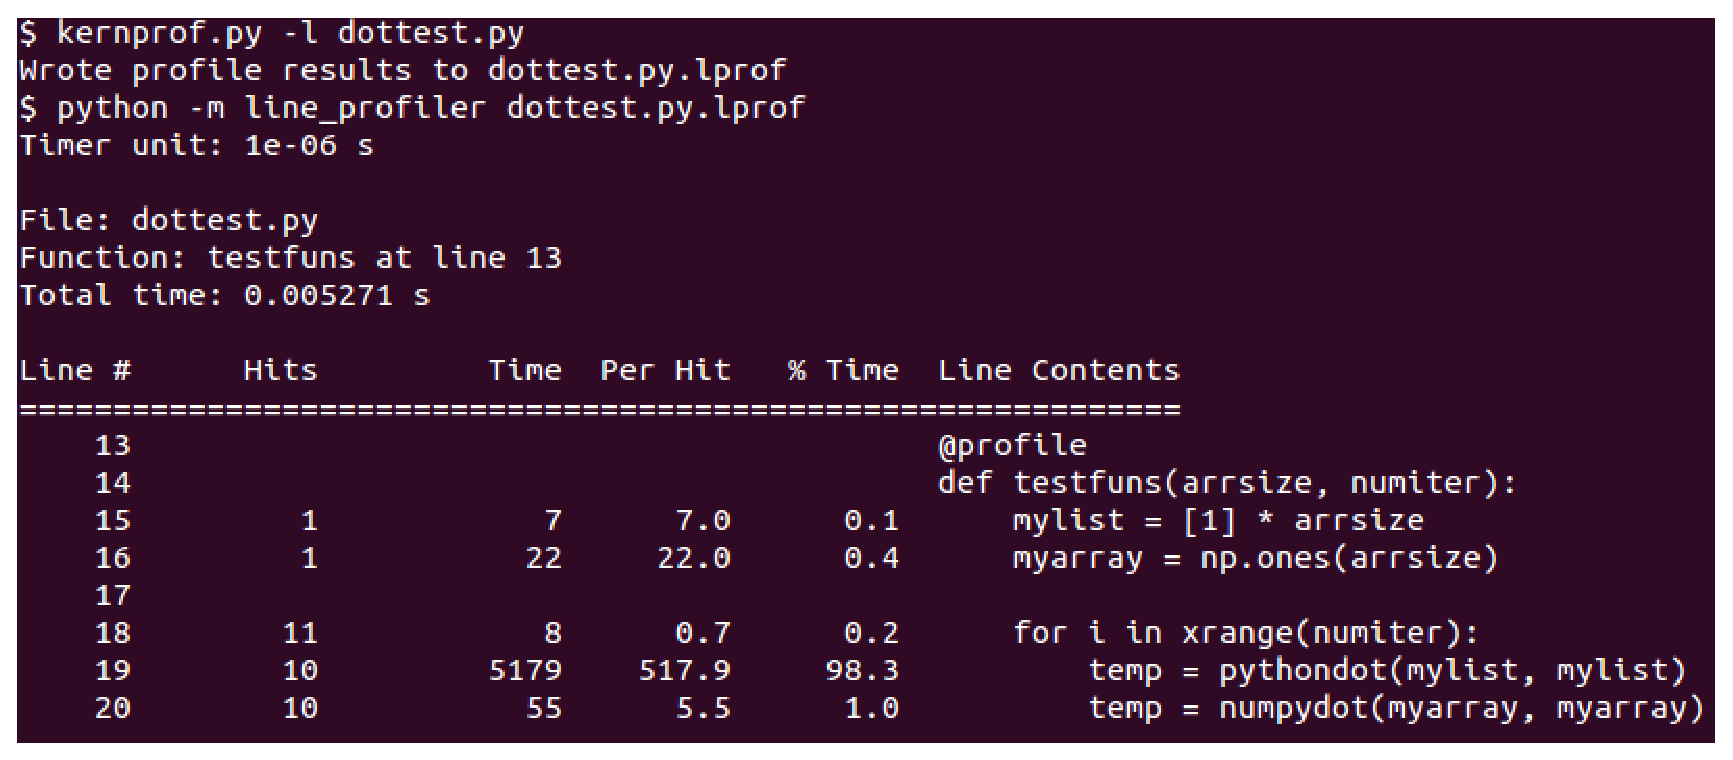
\includegraphics[width=\textwidth]{../images/dottest_profile}
  \caption{Results of profiling session, viewed with less.  See also listing \ref{performance:listing:lineprofiler}.}
  \label{performance:fig:lineprofiler}
\end{figure}
The profile results show the percentage time spent in each function (this is usually the first place I look), the number of times each function was called, and the time spent in each function.  The output in figure \ref{performance:fig:lineprofiler} shows that the pure-python for-loop dot product is much much slower than a numpy dot product.

\subsection{Standard Python rules of thumb}
\label{performance:subsection:rulesofthumb}
Here we go over some standard Python performance tricks and rules of thumb.  These are ``standard'' in the sense that most developers know of them.

\subsubsection{List comprehensions and map}
As evidenced in figure \ref{performance:fig:timeit_1}, a list comprehension is often faster than an explicit for loop.  The reason for this is that a list comprehension handles the append step in an optimized manner.  Thus, if you have a for loop so simple that the appending of an item to a list takes a significant amount of the time, you can get around 50\% speedup.  This 50\% (or so) speed up usually does not merit a pizza party.  So don't be tempted to wrap every for loop into a list comprehension.  This type of code would be unreadable.  A good rule of thumb is this:  If a for loop is not slowing anything down (suppose it is only over a few items), then a for loop is usually more readable and is preferred.  Use a list comprehension only if the list comprehension can be put in one 79 character line.  The \T{map} function is an alternative to list comprehensions.
\begin{minted}{python}
mylist = ...# create a list

def myfun(item):
    ...# do something
    return new_item

# same as [myfun(item) for item in mylist]
myresults = map(myfun, mylist)
\end{minted}

\subsubsection{Hash tables}
Another, sometimes huge, performance tip (that should always be followed) is to take advantage of the fast hash-table lookup capabilities of Python's \T{set} and \T{dict} objects.  Suppose you create a dictionary \T{mydict = \{'name': 'ian', 'age': 13\}}.  A \emph{hash table} is created that stores the keys ``name'' and ``age.''  These keys are not stored as the actual strings.  Instead, they are transformed using a \emph{hash function} to a location in a table.  Many different keys could be transformed to the same location, but it is very very unlikely that this will happen to you.  So you can safely assume that in \T{mydict}, the keys ``name'' and ``age'' are mapped to different locations.  The values (or rather, pointers to the values) are stored at these locations.  So, when I write \T{mydict['name']}, Python uses a hash function to transform ``name'' to a location, and in that location is the string ``ian.''  See figure \ref{performance:fig:hash}.  The performance significance is that, no matter how long your dictionary is, it takes the same amount of time to find a key in it.  For comparisons sake, you could (and many novices do) implement a slow dictionary by storing two lists, one with the keys and one with the values.  Note that a \T{set} is also stored as a hash table (with no values, other than an indication that the element is in the set), so finding items in a set is also fast.  See figure \ref{performance:fig:hash_test}
\begin{figure}
  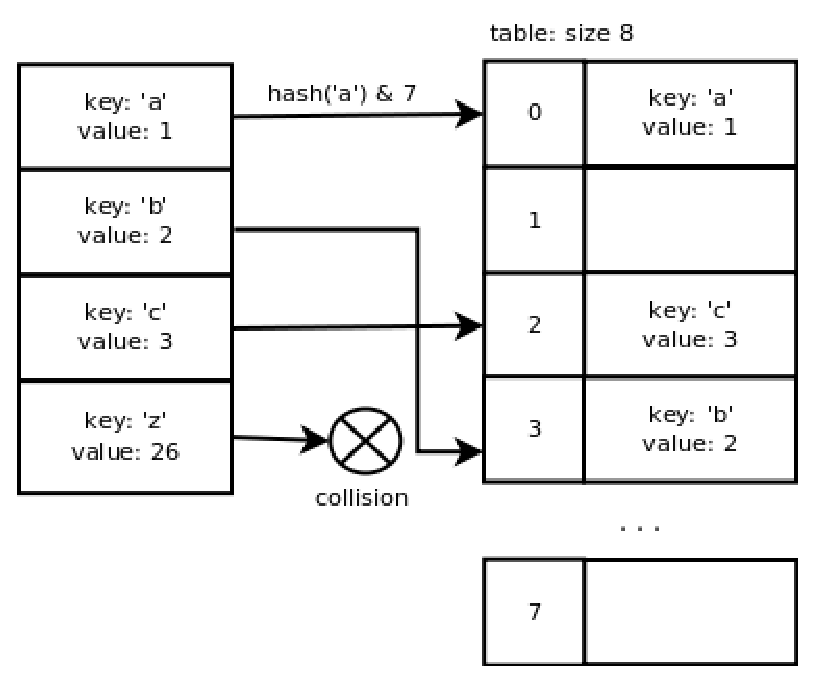
\includegraphics[width=0.75\textwidth]{../images/hash}
  \caption{A hash table corresponding to the dictionary \T{\{'a': 1, 'b': 2, 'c': 3, 'z': 26\}}.  In this table, both \T{'a'} and \T{'z'} were mapped to the same table entry, so there was a collision.  In reality, this is very very rare.}
  \label{performance:fig:hash}
\end{figure}
\begin{figure}
  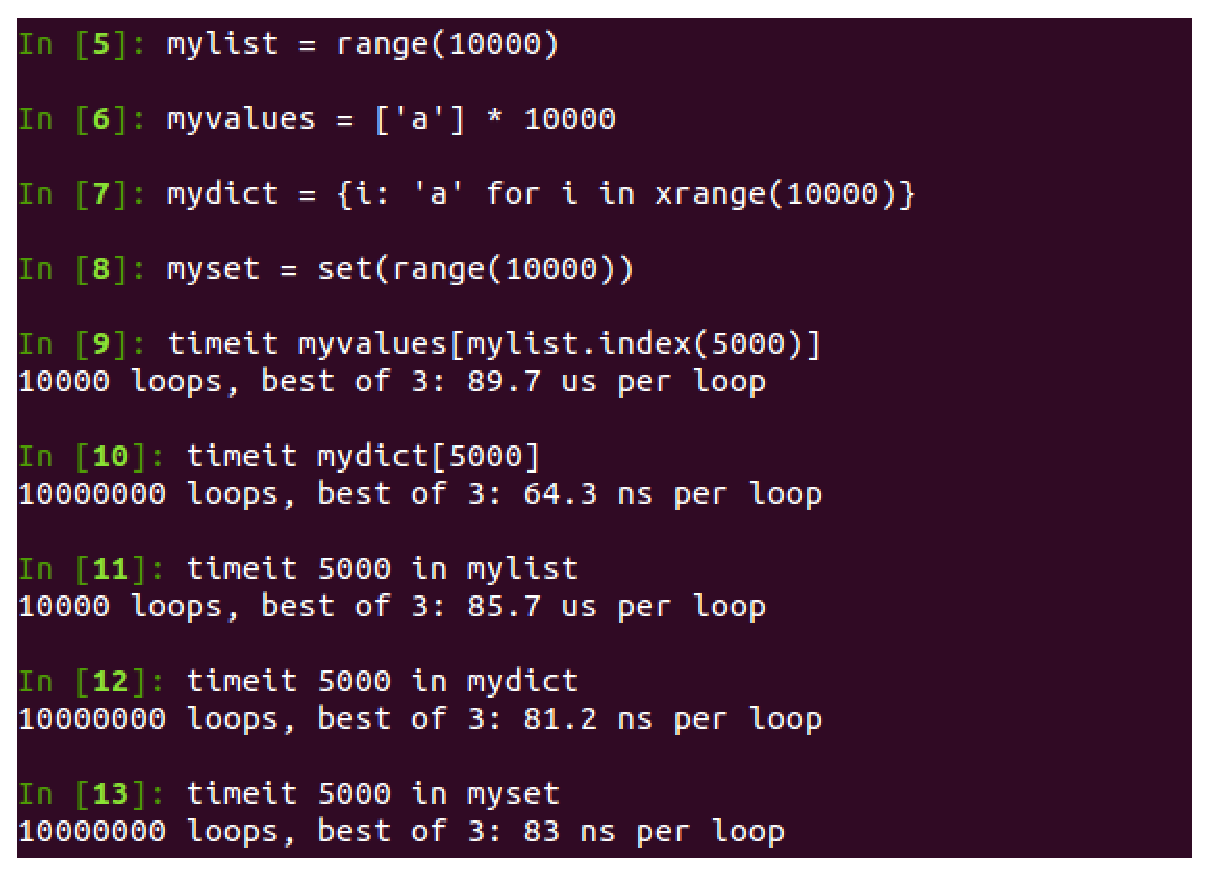
\includegraphics[width=0.85\textwidth]{../images/hash_test}
  \caption{A performance test showing where a hash table is 1000 times faster than list lookup.  Note that \T{mydict} will be a dictionary with keys equal to the numbers 0 through 9999, and every value equal to 'a'.   The calls \T{myvalues[mylist.index(5000)]} and \T{mydict[5000]} both return the 5000th entry in mylist/mydict (equal to 'a' in both cases).  The list version is 1000 times slower because \T{mylist.index(5000)} searches through the list, entry-by-entry, for the number 5000.  The last three calls are boolean tests, each returning \T{True}.}
  \label{performance:fig:hash_test}
\end{figure}

\subsubsection{Iterators}
Consider the following code:
\begin{minted}{python}
mylist = ... # Create a list
for i in range(N):
    mylist[i] = mylist[i] + 10    
\end{minted}
This steps through a list and modifies it.  We use another list, namely \T{range(N)}, to provide an iterator \T{i} to help us step through.  The first time through \T{i=0}, the second \T{i=1} and so on.  You can access the iterator by setting (try it!) \T{myiter = range(10).\_\_iter\_\_()}.
\begin{minted}{python}
>>> mylist = range(10)  # Create a list
>>> myiter = mylist.__mylist__.iter()
>>> myiter.next()
0
>>> myiter.next()
1
\end{minted}
This is more-or-less what happens when you use \T{for in range(10):} to do ten iterations of some task.  This is somewhat wasteful however since we never actually need the entire list at once.  All we need is some way to step through the numbers that would have been in the list.  This same ends can be achieved by replacing \T{range} with \T{xrange}.  The speed difference between using \T{range} and \T{xrange} is small, but the memory savings can be significant and it is generally good practice in Python 2.7 to use \T{xrange}.  \footnote{Note that in Python 3.0+ \T{range} will automatically be converted to \T{xrange} inside for loops, and \T{xrange} will no longer be used\ldots.  So if you want your code to be Python3.0+ compliant, use \T{range}.}

In general, an \emph{iterator} is an object with a directed one-dimensional structure and a \T{next()} method that allows us to iterate through that structure.  A \T{list} is an \emph{iterable} since it can be converted to an iterator.  A \emph{generator} is an iterator that is tied to a function (so that some function is called to provide the next element).

List comprehensions can be replaced with expressions that produce iterators that have a \T{next()} method.
\begin{minted}{python}
>>> mylist = ['a', '0', 1, 'b']
>>> mygen = (item for item in mylist if item.isalpha())
>>> mygen.next()
a
>>> mygen.next()
b
>>> mygen.next()
Traceback (most recent call last):
  File "<stdin>", line 1, in <module>
StopIteration
\end{minted}

A common use of iterators that we have made extensive use of is the file object.
\begin{minted}{python}
>>> f = open('myfile.txt', 'r')
>>> f.next()
'this is the first line\n'
>>> f.next()
'this is the second line\n'
\end{minted}
Note that you could read the entire file into memory at once using \T{f.read()} or \T{f.readlines()}.  This however is often a very wasteful use of memory.

\begin{exercise}
  Consider the following code fragment that loops through using an explicit index:
  \begin{minted}{python}
mylist = ... # Create a list
mysum = 0
for i in xrange(len(mylist)):
    mysum += mylist[i]
  \end{minted}
In contrast, consider this method of looping, which does not use an index:
  \begin{minted}{python}
mylist = ... # Create a list
mysum = 0
for item in mylist:
    mysum += item
  \end{minted}
  The second method works if \T{mylist} is replaced by an iterator, but the first method does not, why?  

  Note that this is a reason the second method is preferred.  If you also need the index, then try using \T{for i, item in enumerate(mylist)}.
\end{exercise}

\subsection{For loops versus BLAS}
\label{performance:subsection:forblas}

As figure \ref{performance:fig:lineprofiler} shows, dot products are much faster in numpy than in pure Python.  The reason that numpy is fast is that it uses some version of the Basic Linear Algebra Subprograms (BLAS).  BLAS is a library of linear algebra functions, mostly written in Fortran.  It takes advantage of your machine's cache configuration, and some versions support multi-threading.  The version of BLAS that comes with standard numpy is 5 - 50 times slower than an optimized version, so the user is encouraged to upgrade to a version that is built with an optimized BLAS (i.e. Intel's Math Kernel Library (MKL)).  This is easy to do if you are using Continuum's Anaconda or Enthought's EPD.  There are many reason's that Python for loops are slow.  Consider the following loop:
\begin{minted}{python}
mylist = ... # Create a list

mysum = 0
for item in mylist:
    mysum += item
\end{minted}
Since Python is not compiled, the python interpreter needs to convert this code into machine code every time through the loop.  Moreover, since a list can contain a very wide variety of objects, Python needs to figure out how to add these objects (or if they even can be added) every time through.  Python also checks if you are using a value of \T{i} that is outside the bounds of \T{mylist}.  None of these checks need to be done with numpy arrays since they are of pre-determined shape and data type.  Note that it is \emph{not} efficient to use a for loop on a numpy array (in fact, it is often slower than a list).  Numpy is only optimal when you call the built-in numpy functions (e.g. \T{sum}, \T{dot}, \T{max}) that call external BLAS libraries.

\subsection{Multiprocessing Pools}
Many embarrassingly parallel tasks can be thought of as applying a function to a list, and getting back another list.  Consider first the following (serial) code:
\begin{minted}{python}
mylist = ...# create a list

def myfun(item):
    ...# do something
    return new_item

# same as [myfun(item) for item in mylist]
myresults = map(myfun, mylist)
\end{minted}
So long as \T{myfun(mylist[i])} is independent of \T{myfun(mylist[j])}, this code could be parallelized by 
\begin{enumerate}
  \item Splitting \T{mylist} up into chunks
  \item Sending each chunk to a separate worker process (hopefully attached to a separate processor core)
  \item Letting each process handle its chunk, creating a shorter version of \T{myresults}
  \item Send the results back to the master process, which re-assembles it.
\end{enumerate}
The following code does just that:
\begin{minted}{python}
from multiprocessing import Pool

# Start 4 worker processes
pool = Pool(processes=4)
myresults = pool.map(myfun, mylist)
\end{minted}

If you use \T{pool.map()}, the workers complete their work, then return the results.  This can cause memory issues if the results are large.  A variant is \T{pool.imap()}, which creates an iterator such that results are sent back as soon as they are available.  See section \ref{performance:subsection:stream-processing-text} for more details and an example.

\subsection{Multiprocessing example:  Stream processing text files}
\label{performance:subsection:stream-processing-text}

A common data science task is to read in a large file (that does not fit into memory), compute something with every line (e.g. count word occurrences), and write the results to a new file.  The proper way to do this is to read the file in  line-by-line and process each line one at a time.  This avoids blowing up your memory, and is parallelizable (see below).  

\subsubsection{Serial examples}
An example is the following:
\begin{minted}{python}
def process_line(line):
    # Write some code here
    return newline

with open('myfile.txt', 'r') as f:
    with open('outfile.txt', 'w') as g:
      for line in f:
          newline = process_line(line)
          g.write(newline)
\end{minted}
A closely related problem would be that of opening many small text files, computing something in each, and printing results to a new file.  As a concrete example, consider the case where we have a collection of files and want to count the occurrences of nouns in them.  To detect nouns requires some non-trivial (and often slow) NLP.  This means that the processing function is likely the bottleneck.  In that case it makes sense to parallelize things.  Let's start with the serial version of this program.

\rule{\textwidth}{2pt}
\begin{minted}{python}
import nltk
from os import listdir
from os.path import isfile, join
import sys


def main():
    basepath = '/home/langmore/jrl/enron/data/raw/enron-spam/all'
    allfiles = [f for f in listdir(basepath) if isfile(join(basepath, f))]

    # The part of speech that we will keep
    pos_type = 'NN'

    for filename in allfiles:
        result = process_file(pos_type, basepath, filename)
        sys.stdout.write(result + '\n')


def process_file(pos_type, basepath, filename):
    """
    Read one file at a time, extract non stop words that whose part of speech
    is pos_type, return a count.

    Parameters
    ----------
    pos_type : String
        Some nltk part of speech type, e.g. 'NN'
    basepath : String
        Path to the base directory holding files
    filename : String
        Name of the file

    Returns
    -------
    counts : String
        filename| word1:n1 word2:n2 word3:n3
    """
    path = join(basepath, filename)

    with open(path, 'r') as f:
        text = f.read()
        tokens = nltk.tokenize.word_tokenize(text)
        good_words = [t for t in tokens if t.isalpha() and not is_stopword(t)]
        word_pos_tuples = nltk.pos_tag(good_words)
        typed = [wt[0] for wt in word_pos_tuples if wt[1] == pos_type]
        freq_dist = nltk.FreqDist(typed)

        # Format the output string
        outstr = filename + '| '
        for word, count in freq_dist.iteritems():
            outstr += word + ':' + str(count) + ' '

        return outstr


def is_stopword(string):
    return string.lower() in nltk.corpus.stopwords.words('english')


if __name__ == '__main__':
    main()
\end{minted}
\rule{\textwidth}{2pt}
Notice how in the above code the I/O is all in \T{main()}, and the processing is all in \T{process\_file()}.  This is the standard ``good practice'' of separating interface from implementation.  We have also made the choice (again, good standard practice) to push the processing to a function that deals with one single file at a time.  This sort of choice is usually necessary for parallelization.

\subsubsection{Parallel example}

We now write a parallel implementation.  We will use the \T{Pool} class from the \T{multiprocessing} package.  This provides an easy way to parallelize embarrassingly parallel programs.  \T{Pool} launches a ``pool'' of workers, and automatically divides up the work among them.  The ``work'' must be passed to them in the form of an iterable such as a list.  It is meant to mimic the functionality of the \T{map()} function.  There is one issue with this however in that \T{map()} will get all results at once, and all the results may be too big to fit in memory.  So instead we use a multiprocessing version of \T{imap}.  \T{imap} returns an iterator that allows us to step through the results one-by-one as they become available.  There is an additional parameter \T{chunksize} that specifies the size of chunks to send to/from the workers at one time.  

It will re-use the functions \T{process\_file()} and \T{is\_stopword} verbatim, so we don't re-write them here.  The \T{main()} function is significantly changed and now supports both single and multiprocessing modes.  There is an additional function \T{imap\_wrap()}, along with a couple of re-definitions, which are necessary if we want to exit with \T{Ctrl-C} rather than explicitly killing the process with \T{ps}.

\rule{\textwidth}{2pt}
\begin{minted}{python}
import nltk
from os import listdir
from os.path import isfile, join
import sys

import itertools
from functools import partial
from multiprocessing import Pool
from multiprocessing.pool import IMapUnorderedIterator, IMapIterator


def main():

    basepath = '/home/langmore/jrl/enron/data/raw/enron-spam/all'
    allfiles = [f for f in listdir(basepath) if isfile(join(basepath, f))]

    # Number of slave processes to start
    n_procs = 2

    # The size chunk to send between slave and master
    chunksize = 10

    # The part of speech type that we will keep
    pos_type = 'NN'

    # Construct a function of one variable by fixing all but the last argument
    # f(filename) = process_file(..., filename)
    f = partial(process_file, pos_type, basepath)

    # Construct an iterator that is equivalent to
    # (f(filename) for filename in allfiles)
    #
    # If we are using 1 processor, just use the normal itertools.imap function
    # Otherwise, use the worker_pool
    if n_procs == 1:
        results_iter = itertools.imap(f, allfiles)
    else:
        worker_pool = Pool(n_procs)
        results_iter = worker_pool.imap_unordered(f, allfiles, chunksize=chunksize)

    for result in results_iter:
        sys.stdout.write(result + '\n')


def imap_wrap(func):
    """
    Wrapper for Pool.imap_unordered that allows exit upon Ctrl-C.  This is a fix
    of the known python bug  bugs.python.org/issue8296 given by 
    https://gist.github.com/aljungberg/626518
    """
    def wrap(self, timeout=None):
        return func(self, timeout=timeout if timeout is not None else 1e100)
    return wrap

# Redefine IMapUnorderedIterator so we can exit with Ctrl-C
IMapUnorderedIterator.next = imap_wrap(IMapUnorderedIterator.next)
IMapIterator.next = imap_wrap(IMapIterator.next)
\end{minted}

\rule{\textwidth}{2pt}
It is instructive to run this script on a large collection of files while monitoring \T{htop}.  We see that each core is able to spend most of its time with a full green bar.  This indicates that they are being fully used.  If chunksize is too large, then one core will end up with significantly more work to do, and this slows things down.  This is only really a problem when you're working with a small number of files, and so this doesn't matter.  If chunksize is too small, you risk burdening the processes with the task of pickling and communicating.  No kidding here!  There are many cases where a small chunksize can result in performance that gets worse as you add more cores.  For the files on my computer at this time, \T{chunksize = 10} was a decent compromise.  In any case, you simply must test out the time with a few different settings to make sure you get some speedup.  This can be done with \T{time python streamfiles.py > /dev/null}.  The redirection sends the output \T{/dev/null}, which is a ``file'' that is erased as soon as it is written.  In other words, you never see the output.

\subsection{Numba}

\subsection{Cython}

